%!TEX root = ../template.tex
%%%%%%%%%%%%%%%%%%%%%%%%%%%%%%%%%%%%%%%%%%%%%%%%%%%%%%%%%%%%%%%%%%%%
%% chapter4.tex
%% NOVA thesis document file
%%
%% Chapter with lots of dummy text
%%%%%%%%%%%%%%%%%%%%%%%%%%%%%%%%%%%%%%%%%%%%%%%%%%%%%%%%%%%%%%%%%%%%

\typeout{NT FILE chapter4.tex}%

\chapter{Proposal}
\label{cha:proposal}

This section defines all our approach for microservice contract evolution.
The compatibility verification, adaptation approach, and benchmark platform will all be described.

\section{Scope} % (fold)
\label{sec:scope}

The proposed solution will support HTTP contracts, because
most applications require a web presence and
microservice teams prefer to use a single protocol for both internal and external communications.

Other event-driven and request-response protocols, such as RPC,
have simplified contracts, and there are already a number of tools that support the evolution of schemas for these protocols,
albeit with some limitations.

\section{Adaptation Approach} % (fold)
\label{sec:adaptation_approach}

The adaptation approach was already introduced, now we will give a more detailed description.
The evolution of contracts is supported by lightweight proxy's capable of dynamically adapting messages exchanged between services to match them with the static service code.
To support this mechanism we will need tree ingredients, a contract description language, a compatibility verification and adaptation protocol.

\paragraph{Contract Description Language}

Contracts in web services can be described with the use Web Api Description Languages (WADL).
The OpenAPI specification is the most widely adopted WADL for HTTP services, instead of designing yet another WADL,
we aim to extend the OpenAPI specification to incorporate support for the needs of our approach.

We will use the Json format to represent records in messages.
Json lacks a language for describing schemas, however, the OpenAPI specification supports the description of record schemas in conjunction with the signature of HTTP endpoints.

\paragraph{Compatibility Verification}

Intuitively, compatibility verification determines whether all the edited elements in the system's modules are compatible with the ones effectively used by the remaining modules,
and whether the new modules' requirements are met by the system's existing resources.
An HTTP contract contains the HTTP method, the path, the parameter schema,
and the location of parameters (path, query, header); the proposed compatibility verification supports all of these elements.
Two approaches will be presented for the verification of contracts:

\paragraph{- Approach A.} In a simplified approach, instead of verifying if a new contract version is compatible with all consumer references
the verification process determines only if the new contract is compatible with the previous versions of the producer.

If a new contract contains an endpoint that is incompatible with a previous version, all consumers of that version,
even if they do not use the incompatible endpoint, are unable to use the new version.

The advantage of this approach is that consumer references don't need to be described and documented;
the verification only processes the producer's new contract and its previous versions.

The disadvantage of this approach is that there are deployments that are deemed unsafe despite being safe.
One way to reduce false negatives is to detect unused endpoints through system log analysis and ignore unused endpoints
when performing compatibility checks.

\paragraph{- Approach B.} In an alternative approach, the verification processes both the producer contract and all the consumer references in each endpoint for
assessing the safety of a deployment operation.

The advantage of this approach is that are no false negatives when accessing the safety of deployments.

The disadvantage is that developers will face an additional burden because consumer references will need to be documented.

\paragraph{}

The compatibility of endpoints and references is typically accomplished via the comparison of element names.
Elements with the same name are considered to be the equal.
In this case, some ambiguous evolutions can only be solved with human intervention and knowledge of the domain.
For example: renaming two fields of the same type; inserting a new field and removing another of the same type, is indistinguishable from renaming a field.
To solve this problem without requiring human intervention,
all elements must be tagged with an immutable and unique key,
and the verification process must use element keys rather than element names.
Low-code visual language editors, such as the OutSystems platform \cite{golovin2017outsystems}, can manage element keys transparently and automatically;
however, in the proposed approach, tags must be manually inserted in the WADL definitions.

\paragraph{}
In the case of solution A. the compatibility verification can be done with human intervention without imposing a significant burden
because it involves comparing only the active versions of one producer.

\paragraph{}
In the case of solution B. the compatibility verification needs to be fully automatic because it involves comparing a new version of a producer, with all consumers.

\paragraph{}

In approach A the verification process automatically outputs a compatibility file for each pair (N,O) where N is the new contract version,
and O is an earlier contract version that is still being consumed.
In this file all mappings between elements in each contract are explicitly defined.
The file can be audited by a developer before it is used in the adaptation protocol.
If the compatibility verification detects an ambiguous case, the developer is notified, and the system only continues after the ambiguity is resolved.

Approach A has an additional advantage over approach B in that it allows for more complex evolution types that can be facilitated with human intervention.
Unlike approach B, which only supports the removal, addition,
and renaming of fields, approach A can accommodate complex contract changes,
such as changing the format of a date, through the use of user-defined adaption functions.

\texttt{e.g.\ new\_contract.startdate = formatDate(earlier\_contract.startdate, format)}

These functions are used in the compatibility file.
Their definition can be provided thorough a static library, or it can be contained within the compatibility file and then executed by mobile code.

This study is leaning toward solution A because, while it produces false negatives, it is a more transparent and flexible approach.

\paragraph{Adaptation Protocol}

The protocol haves two responsibilities, assuring the safety of deployment operations and adapting messages so that they conform with the static service code.

The safety of deployment operations is assured with the help of a service registry that provides a
procedure that employs the compatibility verification described above when a deployment operation is performed.
If the compatibility verification fails, the deployment operation is halted.
To simplify the compatibility verification mechanism, the service registry stores all service contracts and dependencies.
The contracts of services are inserted in the registry when the service is successfully deployed, and removed when the service is discontinued.

The adaptation of messages is supported at runtime by a generated proxy component that dynamically adapts the data exchanged between services.
The proxy adapter intercepts and evaluates all the outgoing and incoming TCP requests to determine whether
they should be left unchanged or how they should be transformed.
The proxy will be installed in both consumers and producers;

When exchanging messages internally the adaption protocol is performed on proxy's installed on consumers,
to avoid centralizing the load of message adaptation in a single point.

When receiving requests from web clients the adaption protocol is performed on the proxy adapter installed in the producer,
in order to keep the endpoints usable by both external and internal clients, while also keeping the evolution of the contract independent.

\paragraph{}

The proxy creation mechanism makes use of the available meta-information present in the service registry
to automatically update the proxy components as needed.
Services are deployed without a proxy, proxies are installed on demand using a lazy instantiation method,
that creates them on the first communication between services.

In essence, every communication contains information about the agreed-upon version, the handshake protocol uses this information to determine if a proxy update is required or not.
The lazy instantiation method improves the maintainability of the system by
simplifying deployment operations.

\section{Benchmark platform} % (fold)
\label{sec:benchmark_platform}

We plan to construct a benchmark platform to compare our solution to existing ones; this section discusses the proposed benchmark platform's requirements and design.

\begin{figure}[htbp]
    \centering
    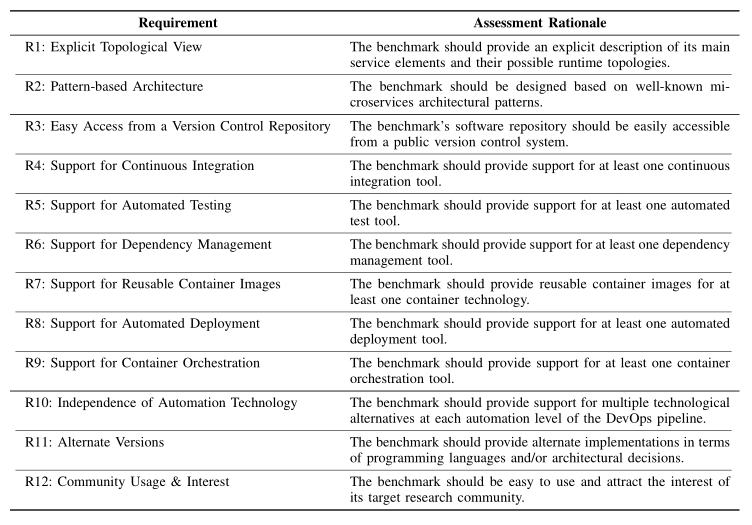
\includegraphics[height=4in]{benchmark_requirements}
    \caption{Benchmark Requirements \cite{microservices2017benchmark}}
    \label{fig:benchmark}
\end{figure}

\citeauthor{microservices2017benchmark} propose an initial set of requirements
to support repeatable microservices research.
In addition to the requirements listed in the ~\ref{fig:benchmark}, the platform's essential requirements are as follows:
\begin{itemize}
    \item The ability to evaluate different solutions in comparable scenarios while utilizing the same evaluation criteria.
    \item Evaluating solutions without requiring modifications to implementations.
    \item Experiments must be simple to share and reproduce by different individuals.
    \item It should be possible to aggregate reported metrics for a specific time period between two events, such as the start and end of a service's evolution.
    \item Users must be able to specify how and when each service should evolve via a configuration file or directly through a terminal.
\end{itemize}

The approaches proposed to be evaluated in comparison to our suggested solution are schema resolution rules, chain-adapter pattern, and traditional versioning.
Each solution will be evaluated in terms of granularity, terminal, type, scalability, maintainability and performance.
\paragraph{}

The architecture of the benchmark platform can be seen in section ~\ref{fig:canvas}.
The architecture components, and their applications are described below:

\paragraph{Kubernetes ~\cite{kubernetes}} will be the test environment.
It will host the services holding the solutions implementations.
The loading testing scripts will also be managed via services in Kubernetes.

\paragraph{Argo ~\cite{argo}} is a robust pipeline engine for Kubernetes, It provides simple, flexible mechanisms for specifying constraints
between tasks and for linking the output of any task as an input to subsequent task.
The argo framework will be used to specify the evolution of services through tasks in an argo workflow,
as well as to manage active virtual users by deploying and stopping docker images that contain load testing scripts.
Complex experiments can be made with Argo since the state of each deployment in Kubernetes can be queried via a task
and utilized as input in a decision that leads to different tasks.

\paragraph{API.guro  ~\cite{apiguro}} is repository of applications Web APIs written in the OpenAPI specification.
The experiments will use the apis available in this repository as a datasets.

\paragraph{OpenAi Generator ~\cite{openapigenerator}} is a tool for generating API client libraries, server stubs, configurations, and documentation from OpenAPI documents.
It will be used to enforce the conformance of tested solution implementations to their OpenAPI contracts.

\paragraph{Promotheus ~\cite{turnbull2018monitoring}} is a pull-based monitoring system.
It periodically sends HTTP scrape requests, the response to this requests is parsed in storage along with the metrics for the scrape itself.
Prometheus provides a query language that allows the metrics to be aggregated by events, components or metadata.
The gathered will be visualized in this platform via Grafana dashboards.

\begin{figure}[htbp]
    \centering
    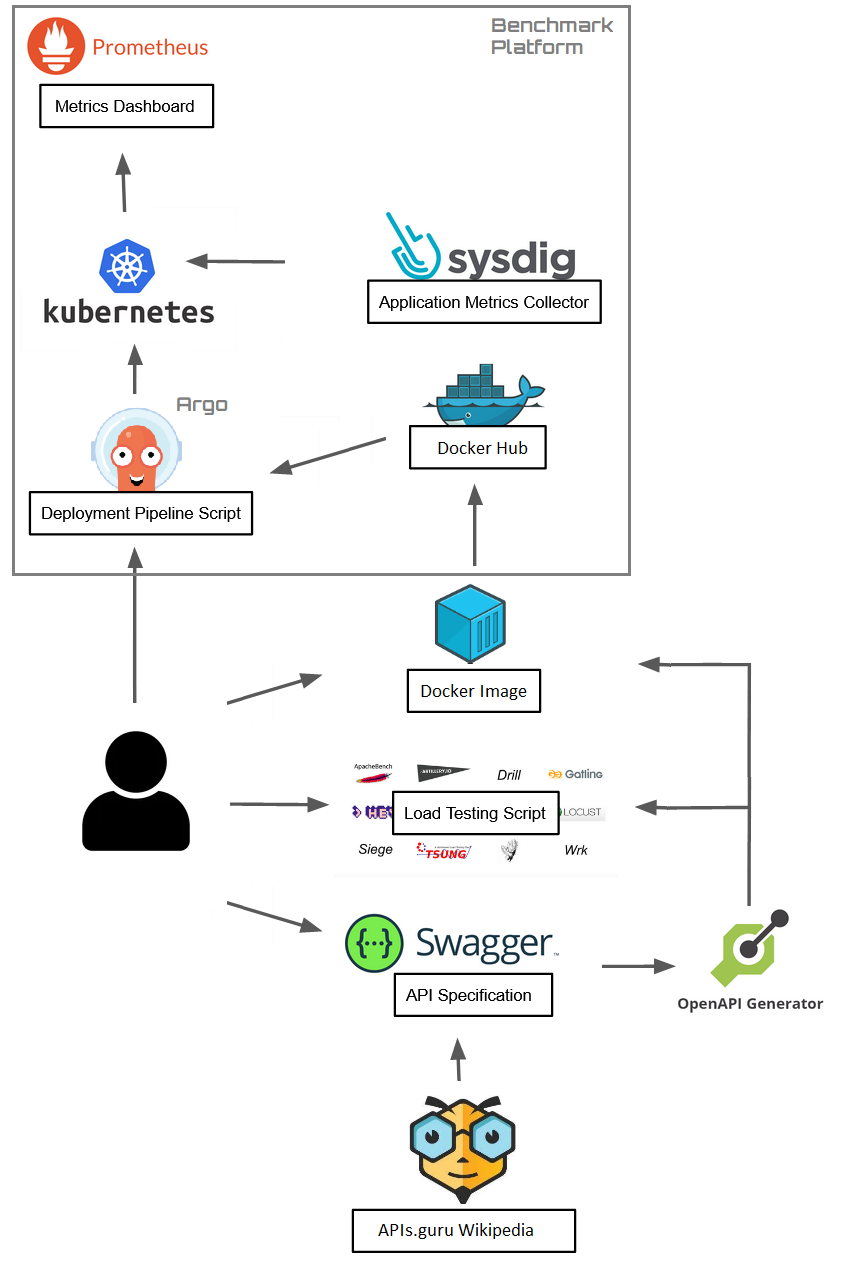
\includegraphics[height=7in]{canvas}
    \caption{Benchmark platform components}
    \label{fig:canvas}
\end{figure}